% !TeX root = ../thuthesis-example.tex

\chapter{相关工作}

\section{模型微调研究现状}

\subsection{预训练技术}

作为迁移学习中最为经典的方法之一,模型微调(Model Fine-tune)的成功离不开离不开模型预训练技术的发展。在深度学习诞生初期,训练数据较少而深度神经网络结构也比较简单,
研究人员往往直接使用基于随机初始值初始化的网络在训练数据上从头开始训练。但是随着数据科学和算力资源的快速发展,这种方式往往需要极其庞大的计算集群连续训练很久很久,对于
普通科研人员以及许多实际场景而言并不现实。Donahue和Oquab~\citep{donahue2014decaf,oquab2014learning}等人的工作发现,训练好的AlexNet提取到的图像特征,可以被迁移到
很多不同的任务中,而且效果明显好于人工设计的特征。这一发现启发了学术界,很多工作~\citep{agrawal2014analyzing,girshick2014rich}也进一步证实,基于预训练的网络参数
进行微调相比完全使用固定的特征提取器能够取得更好的效果。甚至在目标域数据集和预训练数据集完全不同这种更为极端的情况下,模型微调即使无法带来明显的提升~\citep{raghu2019transfusion},
也依然能够加速模型的收敛~\citep{he2018rethinking}。

计算机视觉中卷积神经网络的演变也代表了预训练技术早起的发展,而作为计算机视觉中最为知名的任务,ImageNet-1K~\citep{deng_imagenet:_2009}也成为了预训练技术中最为广泛使用的数据集。
从最早的在ILSVRC2012图像识别竞赛中大放异彩的AlexNet,到通过巧妙设计不断加深网络层数的VGG~\citep{szegedy_going_2015}和引入不同大小卷积核并行结构的Inception Net~\citep{szegedy2016rethinking},
再到使用跳层链接(Skip Connections)实现超深网络结构的ResNet~\citep{he2016deep}和利用密集连接进一步提升效果的DenseNet~\citep{huang_densely_2017},不同结构的深度神经网络在
一次次刷新ImageNet图像分类任务新纪录的同时,也为学术界带来了一个又一个预训练模型。这些基于ImageNet的预训练模型在图像分类、目标检测(Object Detection)、图像识别(Image Recognization)、
语义分割(Semantic Segmentation)等领域都获得了极大的成功。

尽管一直以来的经验认为,网络的深度对模型的性能至关重要,但是深度残差网络(Deep residual network, ResNet)中作者发现,随着深度神经网络深度的增加,
网络的准确度反而达到瓶颈甚至下降,出现了所谓网络退化的现象。作者认为,网络深度的增加会使得网络的容量(Capacity)增大,使其更不容易学习。为了解决退化问题,作者引入了残差机制,对于某个
输入$x$以及其经过网络层后得到的输出$H(x)$,残差学习的目标是学习$F(x)=H(x)-x$这一残差项,那么原始要学习的特征便是$F(x)+x$。当残差为$0$时,网络层的行为就是恒等映射,至少不会使网络的性能下降;
而残差不为$0$时,便意味着网络层在输入$x$的基础上学习到了新的特征。残差结构~\ref{fig:residual}如图所示。ResNet通过引入残差学习的机制,成功将网络深度大幅拓展,也在各类计算机视觉任务中刷新了最好效果。

% 图~\ref{fig:densenet}为DenseNet的示意图。

\begin{figure}
    \centering
    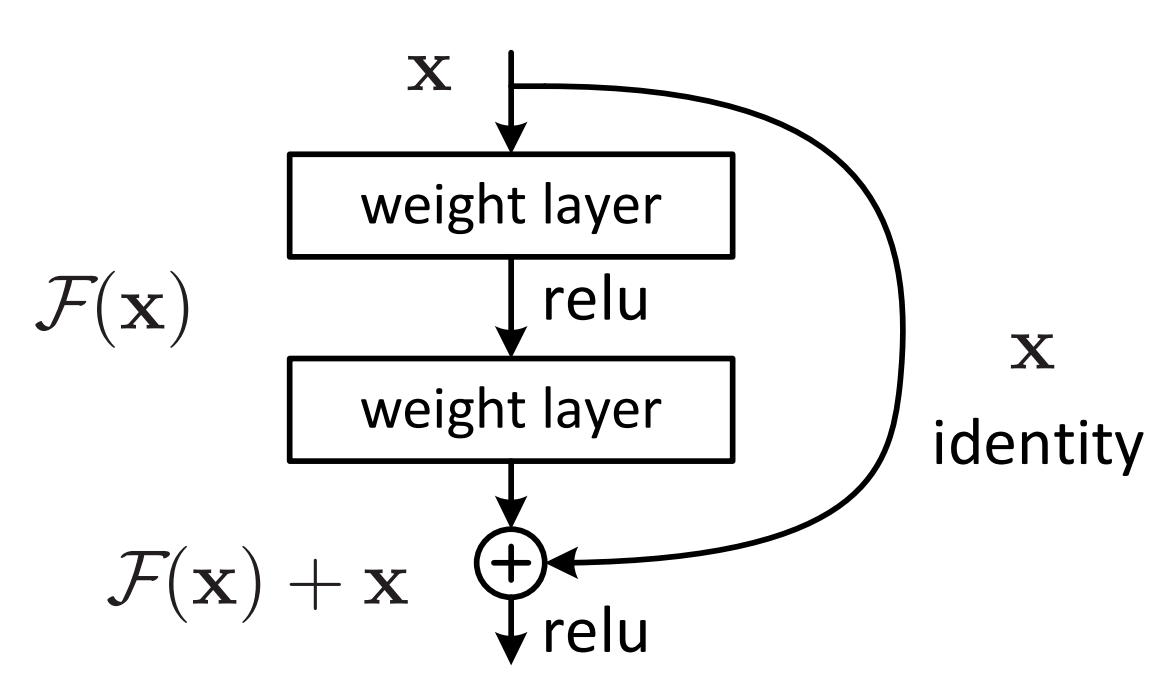
\includegraphics[width=0.5\linewidth]{figures/residual.png}
    \caption{残差结构~\citep{he2016deep}}
    \label{fig:residual}
\end{figure}

深度神经网络的训练技术在自然语言处理(Natural Language Processing,NLP)领域也取得了非常有意义的成果。Word2Vec~\citep{mikolov2013distributed}和Glove~\citep{pennington2014glove}等工作提供了预训练得到的词向量表征,但是在下游任务
中依然需要从头训练更高层级的语义表示。BERT~\citep{devlin2019bert}则通过在掩码语言模型(Masked Language Modeling)上进行预训练,获得了非常强大的预训练表征,使得很大一部分下游任务只需要基于BERT进行微调,就能
取得很好的效果。BERT的结构如图~\ref{fig:bert}所示,它的提出再一次证明了预训练技术的强大与可靠,各种各样基于BERT改进的预训练模型在NLP的各类任务上不断刷新最好成绩。

\begin{figure}
    \centering
    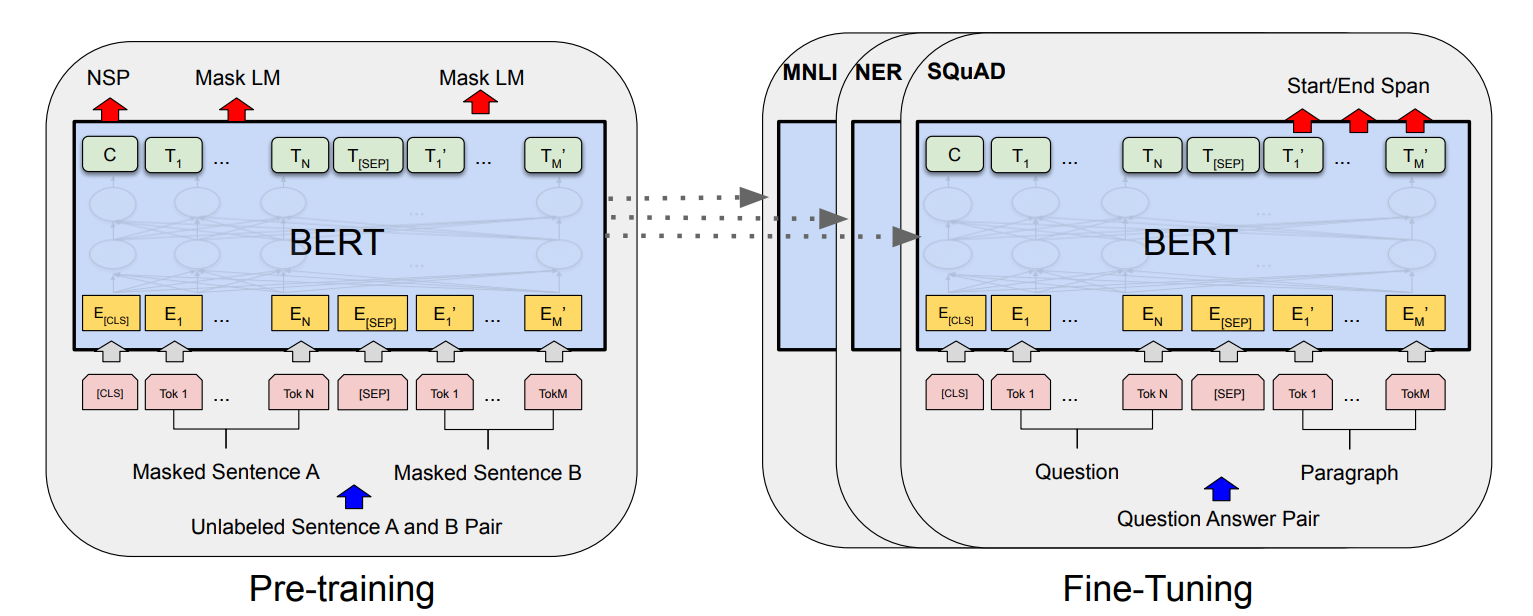
\includegraphics[width=\linewidth]{figures/bert.png}
    \caption{Bert结构~\citep{devlin2019bert}}
    \label{fig:bert}
\end{figure}

图~\ref{fig:bert}为Bert的结构示意图。传统的自然语言处理领域的预训练模型,会受到单向语言模型的限制,只能在一个方向上获得上下文的信息。Bert(Bidirectional Encoder Representation from Transformers)
则顾名思义,是一个双向预训练得到的语言表征(representation)模型。Bert的一种预训练方式是基于掩码语言模型进行的,在预训练序列中以一定概率随机将字符(token)替换为掩码[MASK],再使用模型去预测这些掩码位置对应的字符,
这种方式使得模型不再受单向语言模型的限制,同时对所有的字符都敏感,从而抽取出足够强大的语言表征。Bert可以说是自然语言处理领域最为成功的预训练模型之一,通过基于Bert进行模型微调,在许多自然语言处理任务上取得了当时最好的效果。

传统的基于单一类型数据训练得到的模型,往往会局限于定义好的数据类别中进行预测,一旦遇到从未见过的数据,效果会显著下降。为了解决这一问题,研究人员将目光转向了多模态的预训练模型,希望通过拓展预训练的维度来获得更泛化的预训练模型。
在多模态预训练模型CLIP~\citep{radford2021learning}中,深度神经网络的输入不再是单一的图像数据,而是额外加入了自然语言对图像的描述作为提示信息(prompt),使用这种带有描述的图像进行训练得到的模型具有更好的泛化性,
在小样本学习(Few-shot Learning)、零样本学习(Zero-shot Learning)中有着更好的表现。
图~\ref{fig:clip}为CLIP的结构示意图。

\begin{figure}
    \centering
    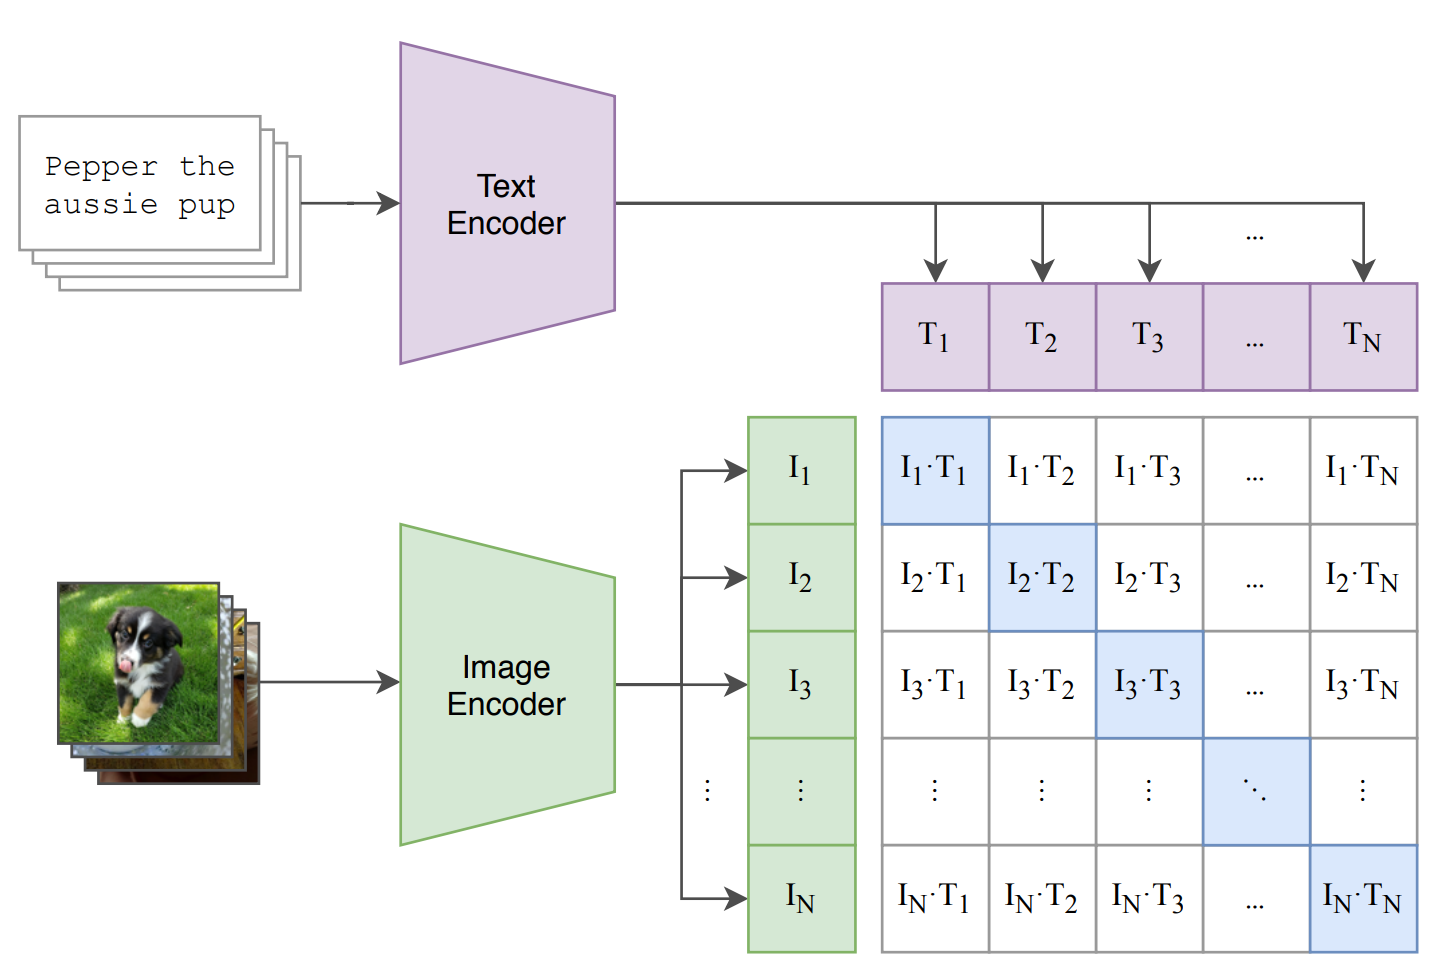
\includegraphics[width=0.8\linewidth]{figures/clip.png}
    \caption{CLIP的结构图~\citep{radford2021learning}}
    \label{fig:clip}
\end{figure}

\subsection{灾难性遗忘与负迁移}

尽管预训练技术的发展为研究人员提供了多种多样预训练模型的选择,但是在模型微调阶段依然会遇到各种各样的困难,其中灾难性遗忘(Catastrophic Forgetting)与负迁移(Negative Transfer)是很常见的两个问题。

依照顺序方式学习任务的能力对于人工智能的发展是至关重要的,然而一直以来对于深度神经网络,灾难性遗忘都是很难避免的。灾难性遗忘是指在新的任务上进行训练时,深度神经网络会逐渐丢失旧任务的相关信息,导致无法
按照预期进行顺序学习,这与网络的连接式结构、网络优化的方式等因素都有关系~\citep{french1999catastrophic}。
模型微调就是一种非常经典的顺序学习范式,在使用目标域数据对预训练模型进行微调时,由于带有标注的训练数据往往非常稀少,导致模型容易逐渐忘记预训练模型中的知识,产生过拟合,
也被称为表征崩坏(representational collapse),体现为原本依靠预训练技术得到表征的泛化性随着训练的进行逐渐减弱~\citep{aghajanyan2020intrinsic}。
研究人员一直以来都在为解决这一问题进行不断的尝试,最简单的方法便是选择较小的学习率并且使用提前停止(early-stopping)的技术,从而避免模型参数更新程度过大。但是这种方法很容易
使得模型陷入局部最优值,尤其是当下游任务差异较大时愈加明显。

\begin{figure}
    \centering
    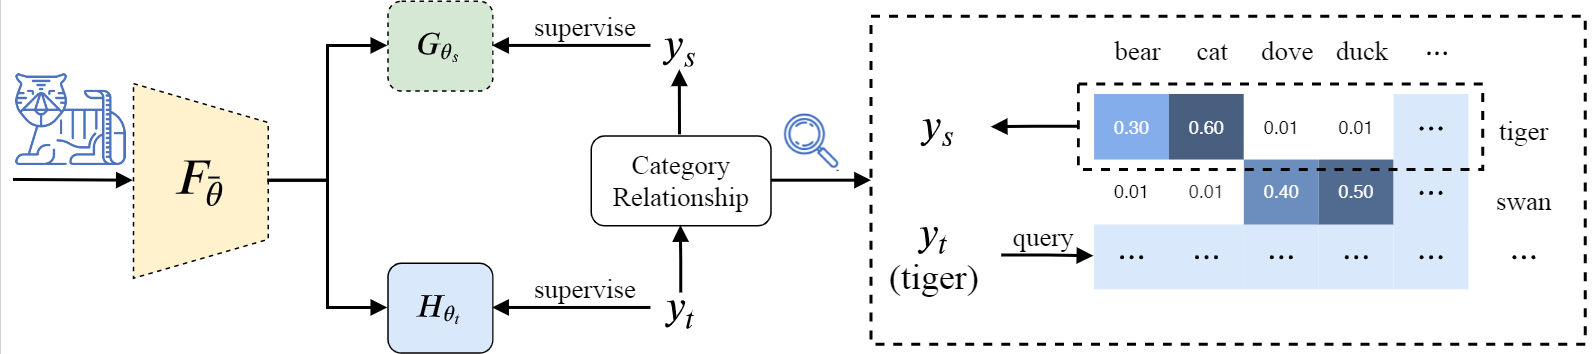
\includegraphics[width=\linewidth]{figures/cotuning.png}
    \caption{Co-Tuning的示意图~\citep{you2020co}}
    \label{fig:cotuning}
\end{figure}

基于正则化约束的模型微调时解决灾难性遗忘的一种经典且有效的方法。
最直接的方式便是直接通过约束网络的预测结果来控制网络的训练,Learning Without Forgetting~\citep{li2017learning}便是其中的代表工作。LWF中认为,在不同域的数据集之间可以共享一个通
用的特征提取器,只需要分别使用各自对应的分类器即可获得很好的效果。由于灾难性遗忘的一大表现是在新任务上获得提升的同时在过去任务上显著下降,因此LWF在新任务上使用新的分类器进行微调的同时,依然保持对所有旧任务分类器的训练。
这种训练范式自然而然地能在保证新任务模型效果的同时不遗忘过去任务中的知识。这种思路也被拓展到了图像分类以外的任务上,取得了不错的效果。
Co-Tuning~\citep{you2020co}则直接利用预训练模型分类器中的知识,建模了源域数据标签空间和目标域标签空间间的映射关系,并利用这一映射关系在模型微调阶段生成伪标签辅助训练,
从另一种角度对网络的预测结果进行了约束,一定程度上避免了灾难性遗忘。Co-Tuning的结构如图~\ref{fig:cotuning}所示。

另一种方式则是通过间接约束网络的参数、特征图等信息,来控制网络的训练。直观上来讲,具有相似参数的网络(层)产生的输出也应该相似,基于这一思想,$L_2$-SP~\citep{xuhong2018explicit}中直接约束特征提取
器的网络参数,避免在模型微调阶段中与预训练模型参数之间差异过大,从而间接约束了网络的输出。而DELTA~\citep{li2018delta}中则选择约束网络中间层输出的特征图,通过注意力机制对特征进行重要性加权,选出
更具有迁移性和判别性的特征。其结构如图~\ref{fig:delta}所示。

\begin{figure}
    \centering
    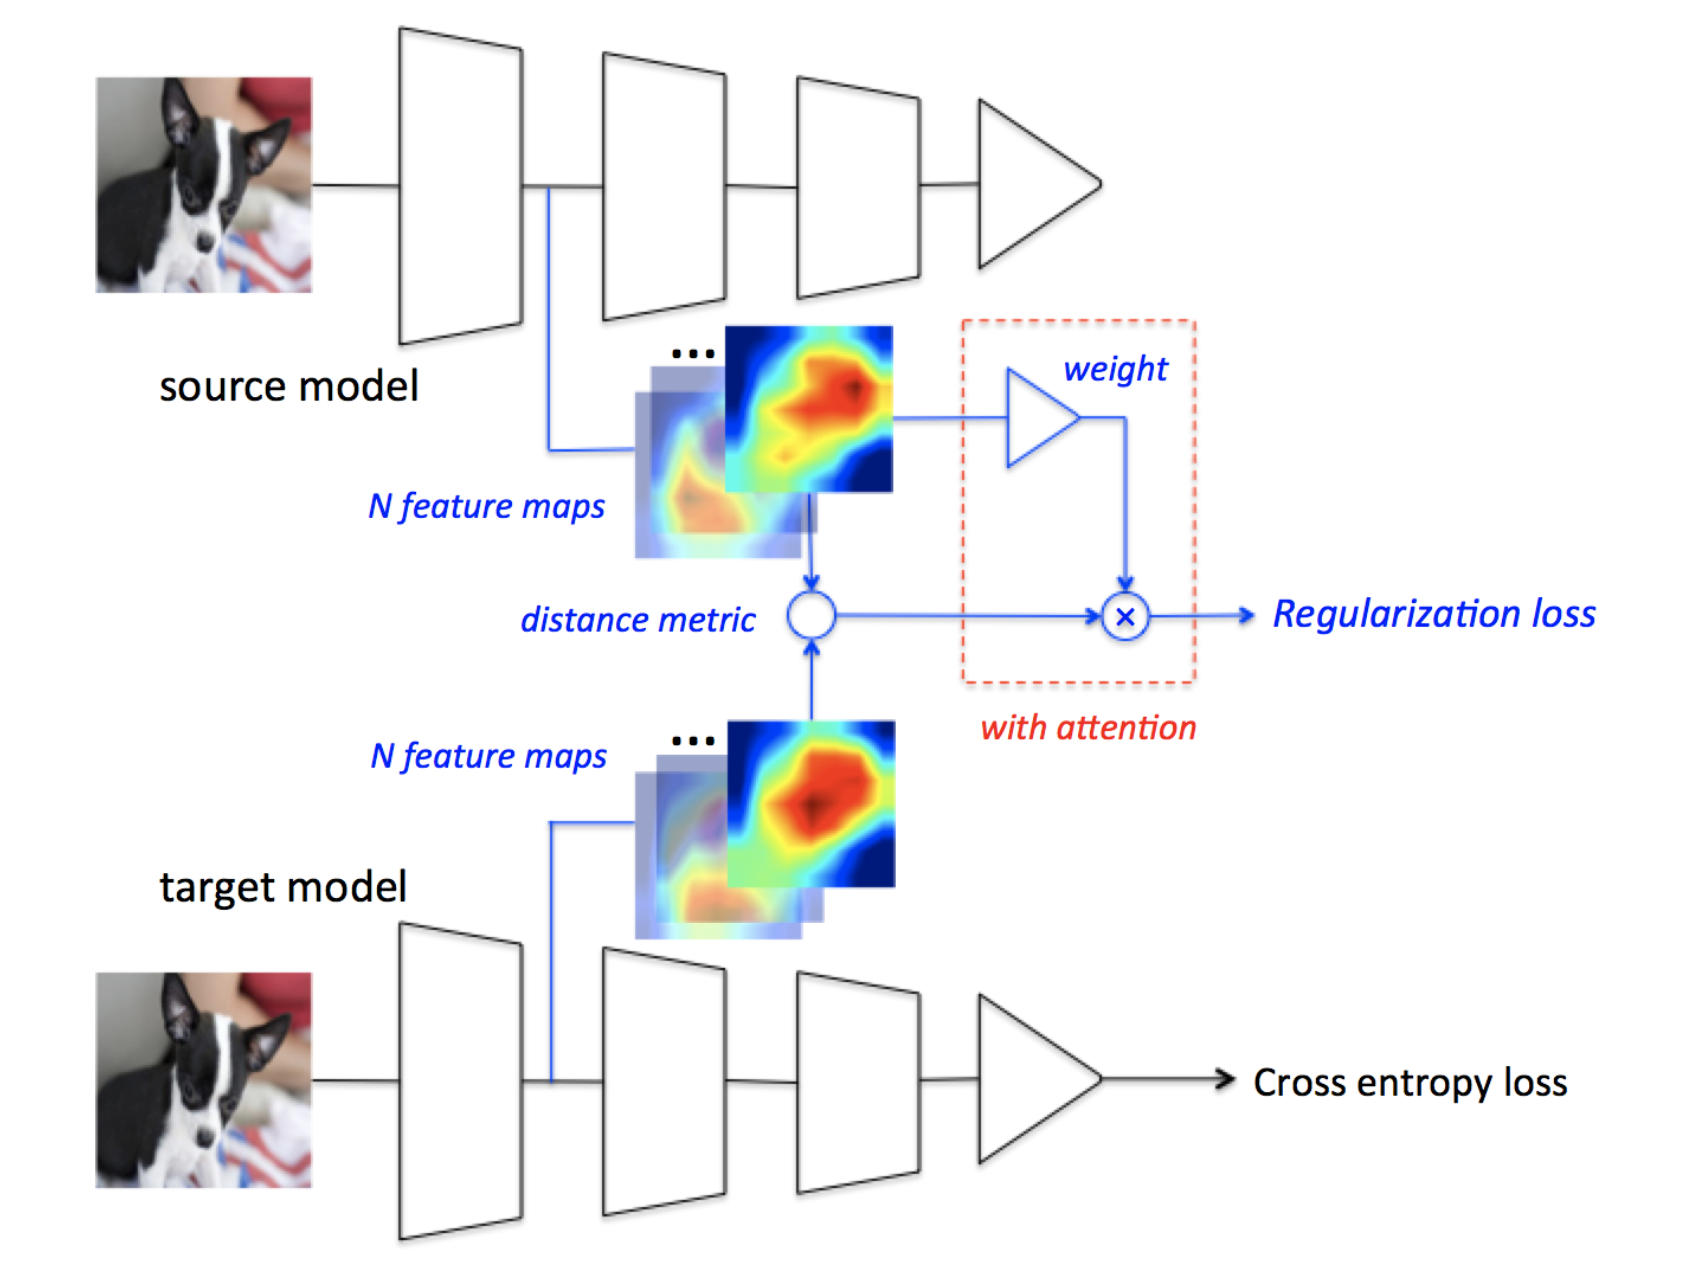
\includegraphics[width=0.8\linewidth]{figures/delta.png}
    \caption{DELTA的示意图~\citep{li2018delta}}
    \label{fig:delta}
\end{figure}

在很长一段时间内,灾难性遗忘都是模型微调领域中非常热门的问题。但是随着研究的深入,研究人员发现在目标域和源域数据差异过大的情况下,过度约束网络的输出、参数以及特征图反而会带来负收益。在BSS~\citep{chen2019catastrophic}中,
作者认为这一现象是因为发生了负迁移。负迁移是指在迁移学习中,由于过度重视预训练模型中的知识而忽略了目标域数据上的特性,迁移了许多不具备迁移性,或者在目标数数据上并不合适的知识,从而影响模型最终效果的现象。

\begin{definition}[负迁移~\citep{wang2018characterizing}]
    令$A(P_s,P_t)$为算法$A$在数据分布$P_s$上预训练得到的模型在数据分布$P_t$上微调得到的模型,$A(\emptyset,P_t)$为在算法$A$在数据分布$P_t$上直接从头训练得到的模型,称
    \begin{equation}
        \mathbb{E}_{(x,y)\sim P_t}[\texttt{Loss}(A(P_s,P_t)(x),y)] > \mathop {\min} \limits_{ A'} \mathbb{E}_{(x,y)\sim P_t}[\texttt{Loss}(A'(\emptyset,P_t)(x),y)]
    \end{equation}
    为负迁移。
\end{definition} 

负迁移在人类的学习任务中也很常见,许多基于经验的知识在面对完全陌生的问题时,往往会让人陷入思维定势。BSS~\citep{chen2019catastrophic}中作者分析了负迁移发生的情况以及原因,并基于谱分析(Spectral Analysis)的技术设计了基于特征图
奇异值分解后得到的奇异值的损失函数,一定程度上避免了负迁移现象的发生。

除了使用约束项避免负迁移外,合理地挑选预训练模型也是解决负迁移的方法之一。早期的研究工作认为任何预训练模型对于下游任务来说都是有益的,但是负迁移现象意味着,当预训练数据与下游任务数据差别过大时,使用这样的
预训练模型会带来负收益。Taskonomy~\citep{zamir_taskonomy:_2018}提出了一种基于任务相关性进行快速挑选的算法;LEEP~\citep{nguyen2020leep}则对预训练数据和下游任务数据标签的联合分布进行预测,利用预测值来衡量预训练
模型的迁移性。但是He等人的工作~\citep{he2021masked}通过实验证明,通过对比式预训练(Contrastive Pre-training)得到的特征在模型微调中的效果并不如生成式预训练(Generative Pre-training),尽管前者具有更好的线性分类
准确率,这意味着预训练模型特征的线性可分性并非评判其迁移性的可靠指标。

\subsection{多模型迁移}

目前学术界的大多数模型微调工作都基于单个预训练模型进行,预训练模型的发展局限于深度神经网络结构的更新。然而随着数据科学的发展,越来越多的预训练数据集被提出,诸如包含了远超ImageNet-1K数据集几个数量级
的ImageNet-21K~\citep{deng2009imagenet}以及JFT-300M~\citep{sun2017revisiting}数据集。预训练任务也不再局限于有监督的图像分类,MoCo~\citep{he2020momentum}和SimCLR~\citep{chen_simple_2020}
尝试利用无监督的训练数据进行预训练,获得了接近于有监督预训练的效果,极大程度上降低了预训练数据的采集难度;He等人的工作~\citep{he2017mask}也提供了在目标检测与实例分割任务上预训练得到的Mask R-CNN模型;
Chen等人的工作~\citep{chen2018encoder}则提供了在语义分割上预训练得到的DeepLab模型。

\begin{figure}
    \centering
    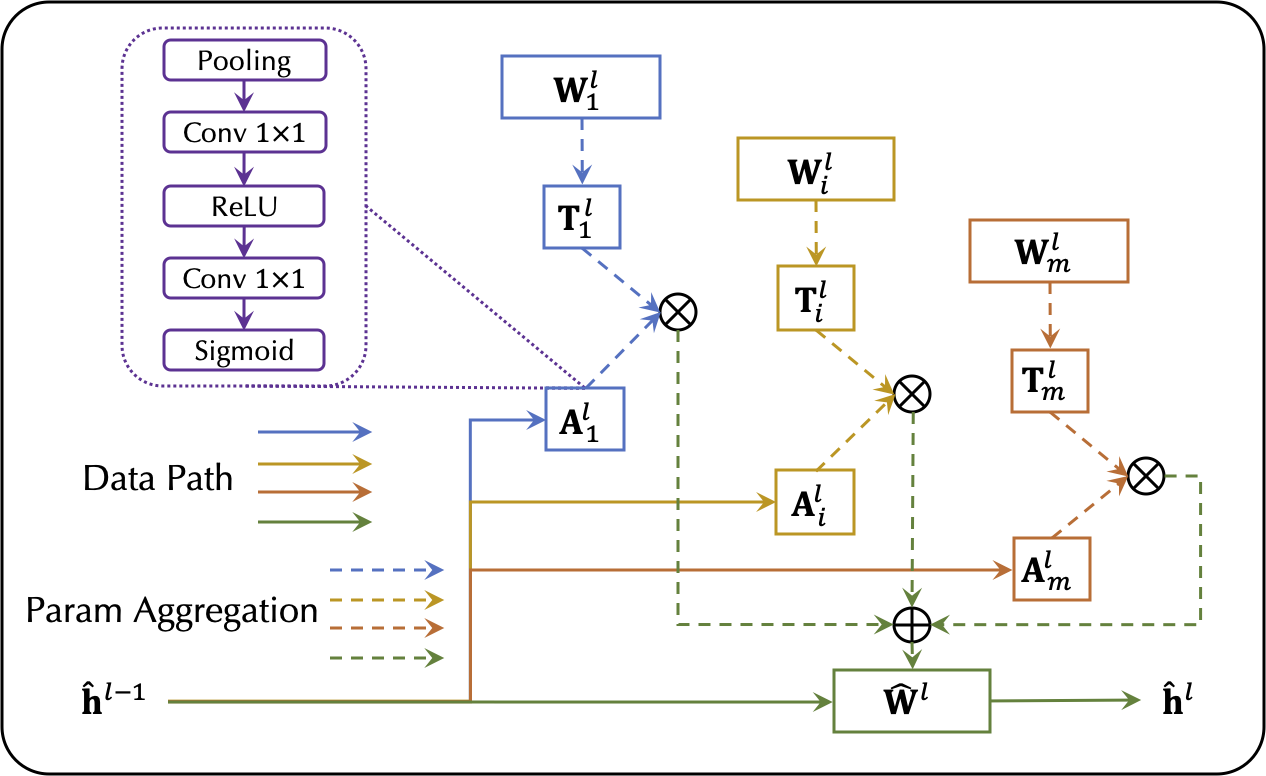
\includegraphics[width=0.8\linewidth]{figures/zootuning.png}
    \caption{Zoo-Tuning的示意图~\citep{shu2021zoo}}
    \label{fig:zoo}
\end{figure}

面对数目众多且任务各不相同的预训练模型,一些工作尝试通过某种机制从预训练模型中选出最适合下游任务的一个进行模型微调~\citep{tran2019transferability,bao2019information,you2021logme},这种方法虽然
将多模型迁移(Multi-model Transfer)与传统的模型微调方法结合了起来,但是仍然有一些不足之处:对预训练模型的筛选机制往往基于某些先验假设,可能并不准确;其次只有一个预训练模型最终被使用,没能充分利用到
如此多预训练模型中的丰富知识。这部分工作还局限于传统模型微调的架构,但是也为之后多预训练模型迁移的研究做出了贡献。一些工作则尝试将不同预训练模型提取的特征进行组合,从而利用预训练模型的先验知
识~\citep{rusu2016progressive,liu2019knowledge},但是这些方法往往需要同时保存多个预训练模型的网络参数,并且要同时提取多种特征,造成了很高的计算和内存消耗。其次,直接使用预训练模型提取的特征而完全
不做针对目标域数据的适应,也很容易在下游任务较为困难,或者和预训练任务有较大的区别时带来负提升。Shu等人的工作~\citep{shu2021zoo}则直接从预训练模型的网络参数角度出发,引入注意力机制计算不同预训练模型
对目标域数据的重要程度,再根据注意力权重对网络参数进行重新组合,从而在不额外增加计算代价的前提下充分利用多个预训练模型中的知识,其结构如图~\ref{fig:zoo}所示。

\section{标准化层}

\subsection{标准化层研究现状}

Boyd等人的工作~\citep{boyd_convex_2004}发现,对输入进行标准化能够对深度神经网络的训练起到帮助,是因为诸如随机梯度下降(Stochastic Gradient Descent,SGD)的一阶优化算法在目标函数曲面更加平滑时效果更好。随后
Ioffe等人的工作~\citep{ioffe2015BN}则提出了批标准化(Batch Normalization)的算法,对网络的输入根据其均值和方差进行标准化,很大程度下帮助了深度神经网络的训练。受BatchNorm的启发,现在深度学习工作中出现了越来越多
的标准化层技巧。层标准化(Layer Normalization)\citep{lei2016LayerNorm}和循环批标准化(Recurrent Batch Normalization)\citep{cooijmans2016recurrent}在循环神经网络的训练中非常有效;组标准化(Group Normalization)
\citep{wu2018GroupNorm}则是为目标检测任务专门设计的;实例标准化(InstanceNormalization)\citep{ulyanov_instance_2016}则提升了风格迁移(Style Transfer)任务的效果。
图~\ref{fig:norm}中展示了这其中的几种标准化层结构的区别。
\begin{figure}
    \centering
    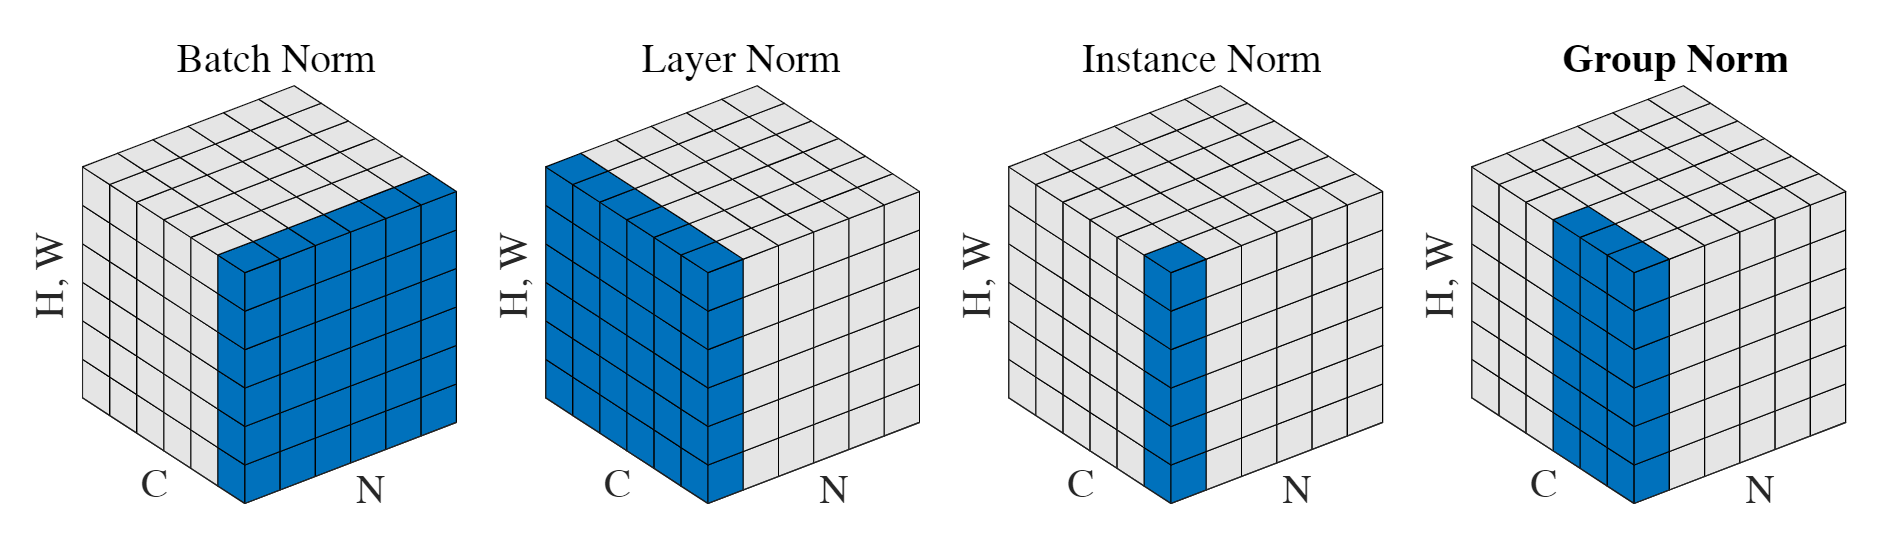
\includegraphics[width=\linewidth]{figures/norm.png}
    \caption{几种标准化层的示意图~\citep{wu2018GroupNorm}}
    \label{fig:norm}
\end{figure}

除此之外,还有一部分标准化层针对深度神经网络的参数进行标准化,例如权重标准化(Weight Normalization)\citep{Salimans2016Weight}则通过简单的重参数化(re-parameterization)
加速了随机梯度下降的收敛速度;谱标准化(Spectral Normalizaiton)\citep{miyato_spectral_2018}则通过约束网络参数的最大特征值从而保证模型满足
1-利普希茨连续(1-Lipschitz continuous),从而避免生成式对抗网络(Generative Adversarial Networks,GAN)中的模型崩溃问题,

\begin{definition}[权重标准化与谱标准化]
    对于深度神经网络中的非线性层以及输入$x$,输出$y$可以表示为:
    \begin{equation}
        y=\phi(\mathbf{w}\cdot \mathbf{x} + b)
    \end{equation}
    其中$\phi$表示激活函数,$\mathbf{w}$为权重向量,$b$为偏移(bias)标量。

    权重标准化中使用与$\mathbf{w}$相同尺寸的向量$\mathbf{v}$和标量$s$对非线性层中的网络参数$\mathbf{w}$进行重参数化,将方向与长度解耦:
    \begin{equation}
        \mathbf{w}=\frac{s}{\vert \vert \mathbf{v} \vert \vert} \mathbf{v}
    \end{equation}

    谱标准化中则直接约束$\mathbf{w}$的最大特征值:
    \begin{equation}
        \begin{aligned}
            \sigma(A) &= \mathop {\max} \limits_{ \symbf{h}:\symbf{h} \neq 0 } \frac{\vert\vert A\symbf{h} \vert\vert_2}{\vert\vert \symbf{h} \vert\vert_2} \\
                        &= \mathop {\max} \limits_{\vert\vert \symbf{h} \vert\vert_2 \leq 1 } \vert\vert A\symbf{h} \vert\vert_2\\
            \hat{\mathbf{w}} &= \frac{\mathbf{w}}{\sigma(\mathbf{w}) } 
        \end{aligned}
    \end{equation}
\end{definition}

本节提到的标准化层都致力于解决各种实际场景下的网络优化问题,而其中在模型微调场景下使用最为广泛的当属BatchNorm,因此本文着眼于卷积神经网络中的BatchNorm进行研究。

\subsection{批标准化层}
\label{section:bn}


批标准化(Batch Normalization)最早由Ioffe等人~\citep{ioffe2015BN}提出,并且被广泛地应用在了很多常用的深度神经网络,诸如InceptionNet~\citep{szegedy_going_2015}和ResNet~\citep{he2016deep}中。同时,这些深度神经
网络也常常被用来当作模型微调的预训练模型使用。

在深度神经网络中,批标准化层以一批(batch)数据的完整特征图(Feature Map)作为输入,输出对其进行批标准化后的结果。值得注意的是,批标准化的操作是在特征图的通道(Channel)维度上进行的,因此本文为了简洁,在公式中省略了通道维度的小标,
只研究一批数据在特征图的某一个通道上进行的批标准化。

给定服从某个分布$P$的特征图$x\sim P$,批标准化的目标是对$x$在批维度通过分布层面(Population-level)的统计值标准化:
\begin{equation}
  \widehat{x}=\frac{x-\mathbb{E}_{x \sim P}[x]}{\sqrt{\operatorname{Var}_{x \sim P}[x]+\epsilon}}
\end{equation}

其中$\epsilon$是一个非常小的常数,用来防止除零。但是分布层面的统计值无法直接计算得到,只能通过在该分布$P$上采样的得到的样本$\{x_{i}\}_{i=1}^{n}$估计得到,其中$n$是数据集的样本数。 

在训练阶段,对于一组批大小为$m$的输入数据$\{x_{i}\}_{i=1}^{m}$而言,首先估计其均值和方差,

\begin{equation}
    \label{eq:mu&sigma}
    \mu=\frac{1}{m} \sum_{i=1}^{m} x_{i},\quad \sigma^{2}=\frac{1}{m} \sum_{i=1}^{m}\left(x_{i}-\mu\right)^{2}
\end{equation}


之后使用计算得到的均值和方差将原数据标准化到均值为$0$,方差为$1$:

\begin{equation}
  \widehat{x}_{i}=\frac{x_{i}-\mu}{\sqrt{\sigma^{2}+\epsilon}}
\end{equation}
  
而在推理阶段,由于输入数据的规模不可控,因此公式~\ref{eq:mu&sigma}的估计方式将不再可行。因此批标准化层在训练阶段通过滑动平均(Moving Average)的方式更新另外一组均值$\tilde{\mu}$和方差$\tilde{\sigma}^2$:

\begin{equation}
    \tilde{\mu} \triangleq \alpha \mu + (1 - \alpha) \tilde{\mu},\quad \tilde{\sigma}^2 \triangleq \alpha {\sigma}^2 + (1 - \alpha) \tilde{\sigma}^2
\end{equation}

作为对分布均值$\mathrm{E}_{x \sim P}[x]$和方差$\operatorname{Var}_{x \sim P}[x]$的估计值,其中$\alpha$表示更新的速率。之后便可以直接用上述的估计值进行标准化:

\begin{equation}
  \widehat{x}_{i}=\frac{x_{i}-\tilde{\mu}}{\sqrt{\tilde{\sigma}^{2}+\epsilon}}
\end{equation}

值得注意的是,这里的$\tilde{\mu}$和$\tilde{\sigma}^2$只在推理阶段参与标准化,对网络的训练没有任何影响。

为了在标准化后恢复特征图的表征能力,批标准化引入了额外的两个网络参数$\beta$和$\gamma$,对标准化后的特征图进行伸缩(Scale)和平移(Shift):

\begin{equation}
  y_{i}=\gamma \widehat{x}_{i}+\beta
\end{equation}


\subsection{批标准化层的局限与改进}
\label{section:problem}

BatchNorm最明显的局限之处在于其均值和方差等统计量的计算都是基于当前batch的输入,因而需要足够大的batch size才能进行准确的计算,但是实际的训练中往往由于计算资源(一般是图形处理器显存)的限制,batch size可能无法满足进
行准确估计的要求。Ioffe等人的工作~\citep{ioffe2017batch}则提出了针对较小的batch size进行训练的批再标准化(Batch Renormalization),用于减弱使用BatchNorm的模型对batch大小的依赖。BatchRenorm的
算法细节如算法~\ref{alg:batchrenorm}所示。
Peng等人的工作~\citep{peng_megdet:_2018}则转向更高效地利用计算资源,提出了跨多个图形处理器的BatchNorm版本,从而获得足够大的batch size来保证BatchNorm的效果。

\begin{algorithm}[htbp]
    \caption{批再标准化 (Batch Renorm)}
    \label{alg:batchrenorm}
    \begin{algorithmic}
        \STATE \hspace{-11pt} {\bfseries 输入}: 一批数据内每个通道的特征图 $x=\{x_{i}\}_{i=1}^{m}$;\\
        (BatchNorm) 滑动平均更新速率 $\alpha \in (0,1)$ 和可学习参数 $\beta, \gamma$; \\
        (Batch Renorma) 滑动平均估计的统计值 $r_{max}$和$d_{max}$。 \\
        \STATE \hspace{-11pt} {\bfseries 输出:} $y={\textrm{BatchRenorm}}(x)$。
    
        \STATE \hspace{-11pt} \textbf{训练阶段:}
        \STATE $\displaystyle \mu \leftarrow \frac{1}{m}\sum_{i=1}^{m}x_{i}, \quad \sigma^2 \leftarrow \frac{1}{m}\sum_{i=1}^{m}(x_i-\mu)^2$ \hfill $//$ \textit{计算均值和方差}
        \setstretch{1.4}
    
        \STATE $\displaystyle r \leftarrow {\texttt{stop\_gradient}}( {\texttt{clip}}_{ [ \frac{1}{r_{max}},r_{max} ] } (\frac{\sigma}{\tilde{\sigma} }) )$
        \hfill $//$ \textit{计算修正后的r}
        
        \STATE $\displaystyle d \leftarrow {\texttt{stop\_gradient}}( {\texttt{clip}}_{[-d_{max},d_{max}]}(\frac{\mu - \tilde{\mu}}{ \tilde{\mu} }) )$
        \hfill $//$ \textit{计算修正后的d}

        \STATE $\displaystyle \widehat{x}_{i} \leftarrow 
        \frac{x_{i}-\mu}{\sqrt{\sigma^2+\epsilon}} \cdot r + d$
        \hfill $//$ \textit{对输入进行标准化}
  
        \STATE $y_{i} \leftarrow \gamma \widehat{x}_{i} +\beta$
        \hfill $//$ \textit{伸缩与平移}
        \STATE $\tilde{\mu} \leftarrow \tilde{\mu} + \alpha (\mu-\tilde{\mu}), \quad \tilde{\sigma}^2 \leftarrow \tilde{\sigma}^2 + \alpha (\sigma^2-\tilde{\sigma}^2)$ 
        \hfill $//$ \textit{滑动平均更新估计值}
        
        \STATE \hspace{-11pt} {\bfseries 推理阶段}:
        \STATE $\displaystyle y_{i} \leftarrow \gamma \frac{x_{i}-\tilde{\mu}}{\sqrt{\tilde{\sigma}^2 + \epsilon}} + \beta$ \hfill $//$ \textit{使用滑动平均估计值进行标准化}
    \end{algorithmic}
  \end{algorithm}

除此之外,BatchNorm在训练和预测阶段使用不同的统计量进行标准化也为其带来了隐藏的问题。Cecilia Summers等人的工作~\citep{summers2019four}中从标准化层输出值的范围对这一问题进行了理论分析,
在训练阶段,由于统计量是在batch内所有样本上计算得到的,此时BatchNorm的输出范围是有界的:

\begin{equation}
    \begin{aligned}
        \mathop {\max} \limits_{ x_1,x_2,\cdots,x_m} &= \gamma \frac{x-\mu}{\sqrt{\sigma^2+\epsilon}} + \beta = \gamma \sqrt{m-1} + \beta \\
        \mathop {\min} \limits_{ x_1,x_2,\cdots,x_m} &= \gamma \frac{x-\mu}{\sqrt{\sigma^2+\epsilon}} + \beta = -\gamma \sqrt{m-1} + \beta \\
    \end{aligned}
\end{equation}

然而在预测阶段,BatchNorm的输出范围是无界的,导致BatchNorm在训练和预测阶段之间存在一定的差异,影响了模型的最终效果。为了解决这一问题,作者提出了预测样本加权(Inference Example Weighting)
的技巧改进BatchNorm:

\begin{equation}
    \begin{aligned}
        \mu &= \alpha \mathbb{E}[x] + (1-\alpha) \tilde{\mu} \\
        \sigma^2 &= (\alpha \mathbb{E}[x^2] + (1-\alpha) \tilde{\sigma}^2) - \mu^2 \\
        \widehat{x}_i &= \gamma \frac{x-\mu}{\sqrt{\sigma^2+\epsilon}} + \beta \\
    \end{aligned}
\end{equation}

其中$m_x$和$m_{x^2}$表示在$x$和$x^2$上进行滑动平均的到的结果。当$\alpha$为$0$时,则退化为标准BatchNorm在预测阶段的计算方式,当$\alpha$为$1$时,则完全依赖预测数据进行标准化,在实际使用中
$\alpha$作为超参数需要通过验证集进行选择,依赖于模型、数据集以及验证指标的选择。

\begin{figure}
    \centering
    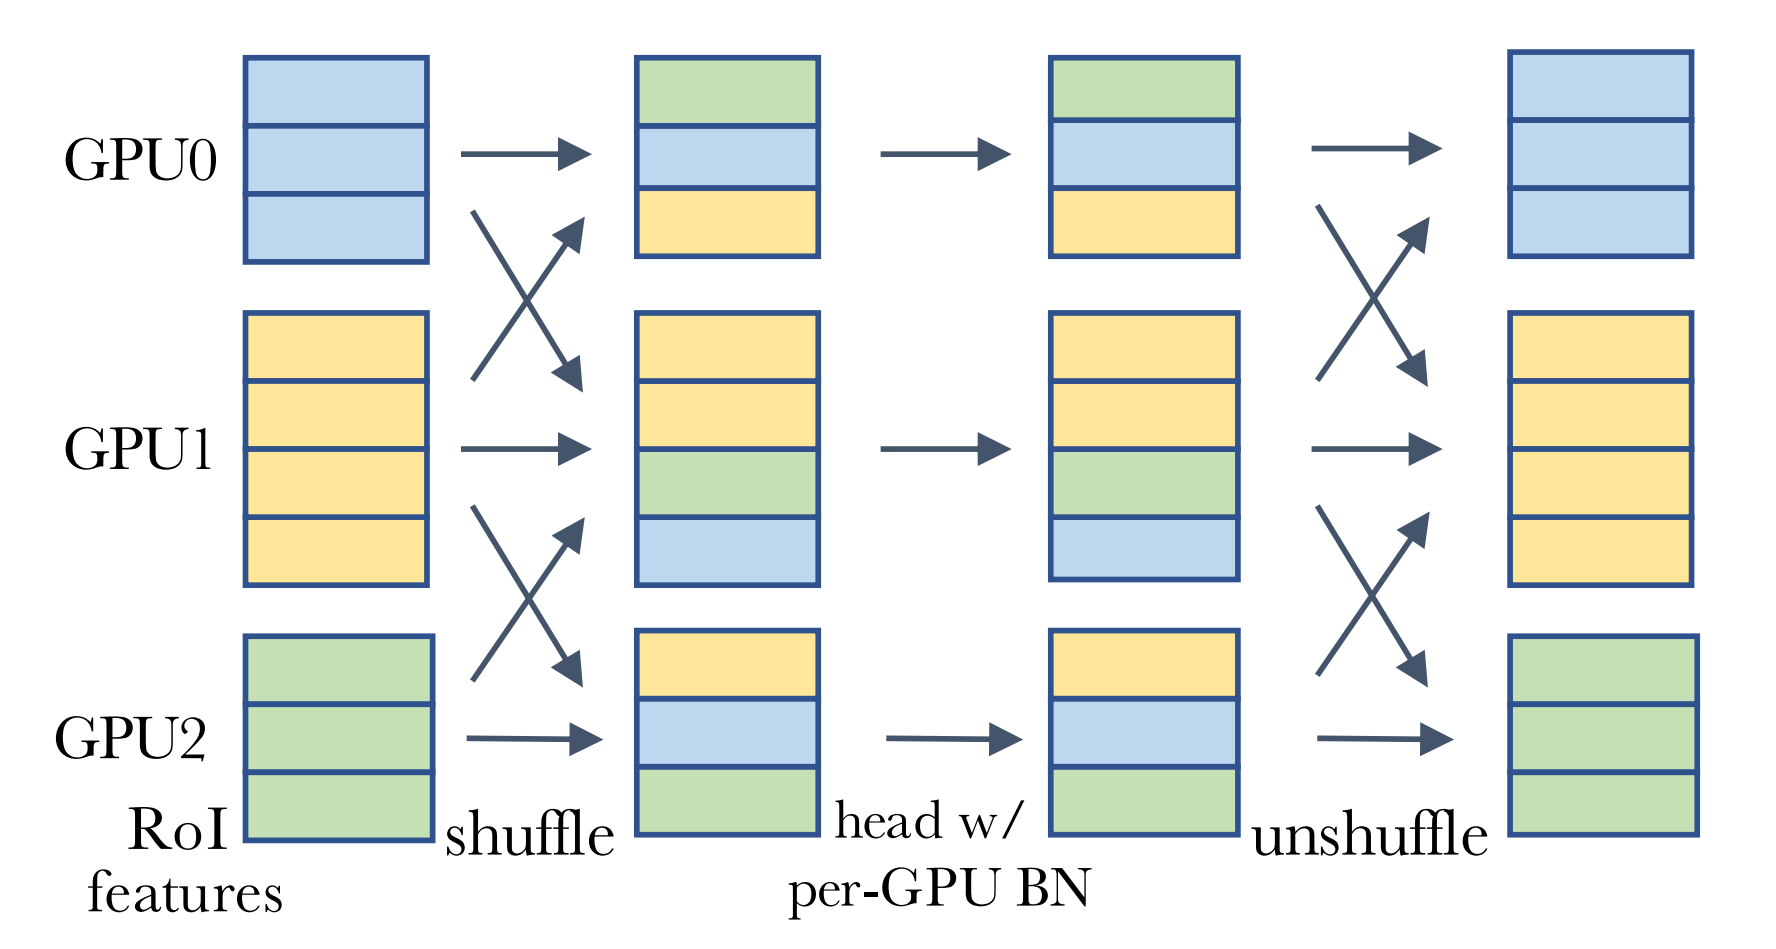
\includegraphics[width=\linewidth]{figures/shufflebn.png}
    \caption{多GPU间的交换批标准化层的示意图~\citep{wu2021rethinking}}
    \label{fig:shufflebn}
\end{figure}

随着无监督预训练的兴起,无监督学习中BatchNorm的不足也开始成为研究人员的关注点。He等人的工作~\citep{he2020momentum}认为,基于对比学习的无监督学习会在同一个batch的数据内部进行对比,而传统的BatchNorm由于在batch内部进行
标准化,会产生一定程度的信息泄露,使得模型容易通过“作弊”找到一种损失函数较小的解,影响模型最终的效果。因此他们提出了交换批标准化(Shuffling Batch Normalization),先交换当前mini-batch内
样本的顺序在进行标准化,最后再将样本顺序复原。他们设计的实验也证实了,在以对比学习为主的无监督学习中,使用交换批标准化能够显著提升最终的效果。

同样的,在Wu等人的工作中~\citep{wu2021rethinking}也提出了这一观点,以多GPU训练的Mask R-CNN模型为例,在预测头中使用标准的BatchNorm会导致结果的下降,这是由于同一个预测头中的样本往往来自同一张图片
的兴趣区域(Region of Interest,ROI),彼此之前存在信息泄露。一种解决方法便是将ROI特征在不同的GPU之间进行交换打散,使得每一个GPU上进行标准化的样本都是全体样本中的一个随机子集,降低了同一个batch内
数据的相关性,图~\ref{fig:shufflebn}为多GPU间的交换批标准化的示意图。

受到这些工作的启发,本文认为标准化层在许多实际应用场景中依然有很大的改进和提升空间,值得进行深入的研究与实验。
